\section{Results}

\subsection{The uTP region combines conserved sequence anchors with a structurally convergent variable domain}

Coale et al. identified a C-terminal extension of approximately 120 amino acids on proteins imported into the nitroplast. We characterized the sequence organization of this extension, hereafter termed the UCYN-A transit peptide (uTP). Two short conserved sequence elements appear at the start of the uTP region in over 90\% of sequences (Figure~\ref{fig:utp_architecture}A). We term these elements anchor 1 and anchor 2 because they mark the boundary between mature domain and transit peptide. Among 745 proteins with detectable sequence elements, 60\% display the canonical order with anchor 2 preceding anchor 1. These anchors are detectable in 80\% of proteins predicted to contain uTP by hidden Markov model search, indicating broad conservation across the import candidate set.

After the anchor elements, sequences diverge into a variable linker region. This region contains additional sequence elements in varying combinations, but shows substantially higher diversity than the anchor region. Pairwise sequence similarity in the linker averages only 7\%, indicating that most uTP sequences share little primary sequence identity beyond the conserved anchors. The linker region varies in length from approximately 50 to over 200 amino acids across different proteins.

Despite this sequence diversity, structure predictions reveal that the anchor motifs encode a conserved three-dimensional fold. We predicted structures for 47 uTP-containing proteins using AlphaFold3. The anchor region adopts a three-helix bundle architecture in 98\% of structures (46/47; Figure~\ref{fig:utp_architecture}B). Anchor 2 forms the first alpha-helix, while anchor 1 folds into a helix-turn-helix motif comprising two additional helices. Together these elements create a characteristic U-bend configuration, with the anchor 2 helix forming one arm and the anchor 1 helix-turn-helix forming the other. Positional variance in this structural core averages less than 1~\AA{} (mean 0.90~\AA{}, range 0.60--1.38~\AA{}), demonstrating strong structural conservation. The high pairwise root mean square deviation across full structures (19.3~\AA{}) reflects variation in linker length rather than divergence of the conserved core.

We next asked whether uTP sequences form discrete subtypes or vary continuously. We applied four clustering methods to uTP sequences: hierarchical clustering, spectral clustering, k-means, and DBSCAN. All methods produced low silhouette scores (0.01--0.08), indicating weak cluster structure. Different methods assigned sequences to completely different groupings, with adjusted Rand indices near zero between methods. Visualization by UMAP shows a continuous distribution with no clear gaps or boundaries (Figure~\ref{fig:utp_architecture}C). Comparison to shuffled controls that preserve amino acid composition confirmed that real sequences show lower silhouette scores (0.096 versus 0.135, permutation test p = 0.01) and lower distance variance (84.6 versus 106.7). This pattern indicates that uTP sequences spread uniformly across a constrained region of sequence space rather than forming discrete subtypes.

The combination of conserved anchors, structural convergence, and continuous sequence variation suggests a model for uTP architecture. The anchor motifs are not merely sequence signatures but structural determinants that encode the conserved three-helix bundle required for recognition by import machinery, explaining their near-universal conservation. The variable linker accumulates mutations freely because it does not participate in recognition. The uniform distribution of sequences in the variable region, with no discrete subtypes, indicates that primary sequence identity in the linker is not under strong selective constraint.

\begin{figure}[!htbp]
    \centering
    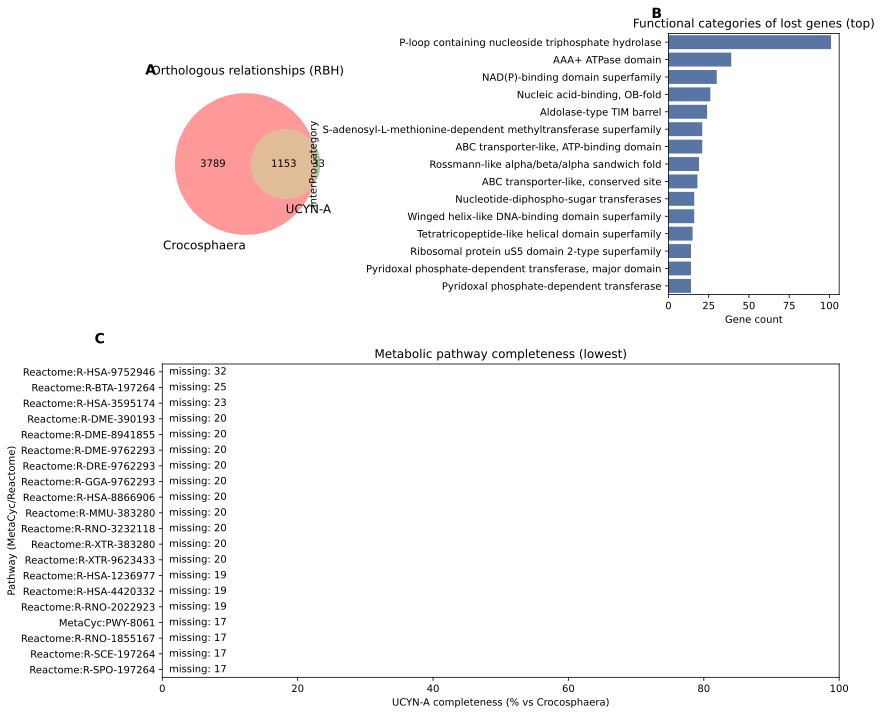
\includegraphics[width=\textwidth]{figures/figure1.pdf}
    \caption[uTP architecture and biophysical signature]{%
    \textbf{The uTP region combines conserved structural elements with a distinctive biophysical signature in mature domains.}
    \textbf{(A)}~Schematic of uTP organization showing the conserved anchor motifs that form a three-helix bundle, followed by a variable linker region.
    \textbf{(B)}~Positional variance along the structural core. The anchor region shows low variance, demonstrating strong structural conservation.
    \textbf{(C)}~UMAP visualization shows a continuous distribution without discrete clusters.
    \textbf{(D)}~ROC curve for predicting uTP presence from mature domain sequences (AUC~=~0.92).
    \textbf{(E)}~Effect sizes for biophysical properties: elevated disorder (+1.05), lower pI (-0.89), and lower instability (-0.81).
    \textbf{(F)}~Within-category effect sizes for intrinsic disorder. All eight functional categories show effects in the same direction.
    \textbf{(G)}~Variance partitioning: uTP status explains more unique variance (7.3\%) than is shared with function (3.4\%).
    \textbf{(H)}~Gene family analysis: 25\% of uTP proteins share families versus 2\% expected, but 624 distinct families with 75\% singletons.
    }
    \label{fig:utp_architecture}
    \end{figure}

\subsection{Mature domain biophysical properties predict uTP presence independently of ancestry and function}

The structural conservation of uTP implies recognition by specific import machinery. We asked whether successful import depends only on the transit peptide, or whether the cargo protein itself must have compatible properties. To test this, we trained classifiers to predict uTP presence from mature domain sequences alone, excluding the uTP region. A logistic regression classifier achieved 92.8\% accuracy in distinguishing uTP-containing proteins from cytoplasmic and nuclear controls (605 versus 773 proteins, permutation test p = 0.002; Figure~\ref{fig:utp_architecture}D). Validation on the full \textit{Braarudosphaera bigelowii} proteome (933 uTP versus 43,430 non-uTP proteins) yielded a receiver operating characteristic area under curve of 0.92, confirming strong discriminative power despite extreme class imbalance.

Three biophysical properties of the mature domain drive this classification (Figure~\ref{fig:utp_architecture}E). First, uTP proteins contain more intrinsically disordered regions than controls (Cohen's d = +1.05, large effect). Second, uTP proteins have lower isoelectric points, indicating greater acidity (d = -0.89, large effect). Third, uTP proteins show lower instability indices, indicating greater thermodynamic stability (d = -0.81, large effect). All three comparisons remain significant after Bonferroni correction for multiple testing.

This finding is unexpected. In canonical protein targeting systems such as chloroplast and mitochondrial import, the transit peptide determines targeting specificity while cargo properties play no role. That mature domain properties predict uTP presence with approximately 90\% accuracy suggests constraints on which proteins can undergo uTP-mediated import.

Two alternative explanations could account for this biophysical signature without invoking cargo-specific selection. First, uTP proteins might share recent common ancestry, with the signature simply reflecting inherited properties from a small number of founder genes. We tested this by clustering all \textit{B. bigelowii} proteins into gene families and asking whether uTP proteins concentrate in particular families. Among uTP proteins, 25\% share a gene family with at least one other uTP protein, significantly more than the 2\% expected by chance (permutation test p < 0.0001). This confirms a contribution from shared ancestry. However, uTP proteins span 624 distinct gene families, and 75\% of uTP proteins belong to families containing only a single uTP member. Shared ancestry contributes to but cannot fully explain the biophysical signature.

Second, uTP proteins might concentrate in functional categories that happen to share these biophysical properties. We assigned proteins to functional categories using COG annotations and compared uTP versus control proteins within each category. If functional enrichment explained the signature, effect sizes should diminish or disappear when comparing same-function proteins. Instead, the biophysical differences persist within categories (Figure~\ref{fig:utp_architecture}F). All eight categories with sufficient sample sizes show the same direction of effect for intrinsic disorder, acidity, and stability. Functional category explains only 0--17\% of the biophysical differences depending on the property. Variance partitioning confirms that uTP status explains more unique variance (7.3\%) than is shared with functional category (3.4\%). The biophysical signature is genuinely associated with uTP status, not an artifact of functional enrichment.

These findings point to dual constraints on uTP-mediated import. The transit peptide must present the conserved three-helix bundle formed by the anchor motifs for recognition by import machinery. The cargo protein must possess compatible biophysical properties: elevated disorder, acidity, and stability. This dual requirement suggests that the evolution of uTP-bearing proteins was shaped not only by the need for a targeting signal but also by selection for cargo properties compatible with transport into the nitroplast.

% Placeholder sections

\subsection{The biophysical signature suggests mechanistic constraints on membrane translocation}

% TODO: This section interprets WHY disorder, acidity, and stability matter
% 
% Paragraph ideas:
% 1. Elevated disorder may facilitate unfolding during membrane translocation
%    - Compare to chloroplast/mitochondrial import where unfolding is required
%    - Disordered proteins unfold more readily
% 2. Acidity (low pI) could mediate electrostatic interactions with import machinery
%    - Positively charged import channels?
%    - Compare to other systems
% 3. Thermodynamic stability may be required for function in the nitroplast environment
%    - Or for surviving the import process
% 4. These constraints are not mutually exclusive


\subsection{Imported proteins complement specific metabolic gaps in UCYN-A}

% TODO: This section covers functional analysis of what gets imported
%
% Paragraph ideas:
% 1. Functional enrichment analysis - what categories are over/underrepresented
%    - Energy metabolism, amino acid biosynthesis enriched
%    - Transcription, trafficking depleted
% 2. Pathway-level analysis - which pathways are completed by host proteins
%    - Threonine, serine, proline biosynthesis
%    - Pyrimidine biosynthesis
%    - Tetrahydrofolate synthesis

\subsection{The uTP system represents a novel protein targeting mechanism}

% TODO: This section compares uTP to other known transit peptide systems
%
% Paragraph ideas:
% 1. C-terminal location is unusual (most transit peptides are N-terminal)
%    - Exceptions: peroxisomal PTS1, some bacterial secretion
% 2. No sequence or structural homologs in databases
%    - BLAST/HMM searches against UniProt, PDB
% 3. Comparison to diazoplast system in Epithemia
%    - Similar nitrogen-fixing organelle, different host
%    - Does it use similar targeting?
% 4. Implications for understanding organellogenesis
